\documentclass[tikz, border=50pt]{standalone}

\usepackage{tikz}
\usepackage{medl_colors}
\usepackage{graphicx}
\usetikzlibrary{shapes.multipart, shapes.geometric, arrows.meta}
\usetikzlibrary{matrix, calc, positioning,fit}
\usepackage{xstring}

\newif\ifmember
\makeatletter
\newcommand{\MemberQ}[2]{\global\memberfalse%
\@for\next:=#1\do{\ifnum\next=#2\global\membertrue\fi}}
\makeatother

\begin{document}
\begin{tikzpicture}

\newcommand\circles[3]
{
    \foreach \i in {1,2,3,4,5,6,7}
    {
    \IfEq{#3}{1}%
        {
            \node [draw=green2, circle, minimum size=.6cm, fill=green0] (circle#1\i) at(#2, -\i+4) {};
        }
        {
            \MemberQ{2,5,6}{\i}
            \ifmember
            {
                \node [draw=green2, circle, minimum size=.6cm] (circle#1\i) at(#2, -\i+4) {};
                \begin{scope}
                \clip(#2, -\i+4) circle(.3cm);
                \foreach \p in {.03, .06, .09, .12, .15, .18, .20, .24, .22}
                { 
                    \foreach \q in {.04, .08, .12, .15, .18, .21}
                    { 
                        \fill (#2, -\i+4) circle (0.01);
                        \fill (#2, -\i+4+\q) circle (0.01);
                        \fill (#2, -\i+4-\q) circle (0.01);
                        \fill (#2+\p, -\i+4) circle (0.01);
                        \fill (#2+\p, -\i+4+\q) circle (0.01);
                        \fill (#2+\p, -\i+4-\q) circle (0.01);
                        \fill (#2-\p, -\i+4) circle (0.01);
                        \fill (#2-\p, -\i+4+\q) circle (0.01);
                        \fill (#2-\p, -\i+4-\q) circle (0.01);
                    }
                }
                \end{scope}

            }
            \else%
            {
                \node [draw=green2, circle, minimum size=.6cm, fill=green0] (circle#1\i) at(#2, -\i+4) {};
            }
            \fi
        }
    }
}

%center part
\node (rect) at (0,0) [draw,fill=pink1, minimum width=1.5cm,minimum height=2cm] (rectangle)  {Bottleneck};

\node[trapezium,
    draw = green2,
    fill = green0,
    text = black,
    align=center,
    trapezium angle=80,
    minimum height=3cm,
    shape border rotate=270,
    left of = rectangle, node distance = 4cm ] (t1) { Encoder};  

\node[trapezium,
    draw = blue1,
    fill = blue0,
    text = black,
    align=center,
    trapezium angle=80,
    minimum height=3cm,
    shape border rotate=90,
    right of = rectangle, node distance = 4cm ] (t2) { Decoder};    

%input
\node[left of = t1, node distance = 4cm, draw=green2, fill=green0, minimum width=1cm,minimum height=8cm ] (input) {};
\circles{1}{-8}{2};
\circles{2}{-10}{2};
\circles{3}{-12}{1};

%output
\node[right of = t2, node distance = 4cm, draw=blue1,fill=blue0, minimum width=1cm,minimum height=8cm] (output)  {};
\circles{4}{8}{1};

%arrows
\draw [-Triangle] (t1.east) -- (rectangle.west) node[midway,right] {};
\draw [-Triangle] (rectangle.east) -- (t2.west) node[midway,right] {};
\draw [-Triangle] (input.east) -- (t1.west) node[midway,right] {};
\draw [-Triangle] (t2.east) -- (output.west) node[midway,right] {};
\draw [-Triangle] ([xshift=1mm]circle34.east) -- ([xshift=-1mm]circle24.west) node[midway,right] {};
\draw [-Triangle] ([xshift=1mm]circle24.east) -- ([xshift=-2mm]circle14.west) node[midway,right] {};

%production system
\node[dashed, draw=orange1, rounded corners, draw, inner xsep = 9cm, inner ysep=6cm] at(0.2, 0) (production){};
\node[below of=production, align=center, node distance=5.5cm] {Production System};

%bottom images
\node[scale = .3, below of = circle17, node distance = 6cm] (inputpic1)  {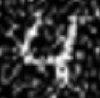
\includegraphics {images/partially_destroyed_input.png}};
\node[scale = .3, below of = circle27, node distance = 6cm] (inputpic2)  {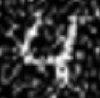
\includegraphics {images/partially_destroyed_input.png}};
\node[scale = .3, below of = circle37, node distance = 6cm] (inputpic3)  {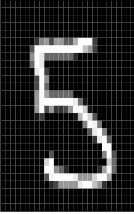
\includegraphics {images/original_input.png}};
\node[scale = .3, below of = output, node distance = 16cm] (outputpic)  {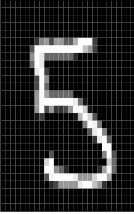
\includegraphics {images/original_input.png}};

%lables
\node[above of=circle11, align=center, node distance=2cm] {Input};
\node[above of=circle21, align=center, node distance=2cm] {Partially\\Destroyed\\Training\\Data};
\node[above of=circle31, align=center, node distance=2cm] (tinput) {Original\\Training \\Data};
\node[above of=output, align=center, node distance=5cm](toutput) {Reconstructed\\Input};


\end{tikzpicture}
\end{document}